\documentclass{standalone}

\usepackage{tikz}
\usepackage{amssymb}
\usetikzlibrary{calc, positioning}
\begin{document}
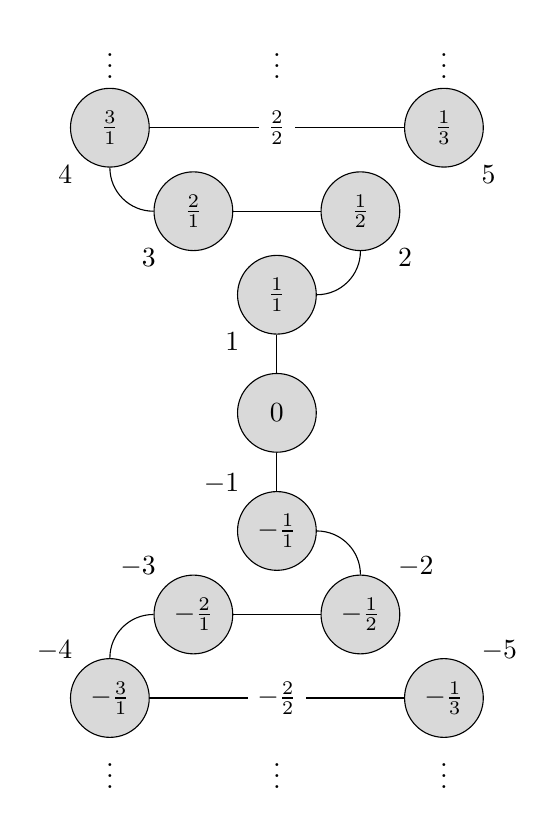
\begin{tikzpicture}[every circle node/.style={minimum size=1cm,draw, fill=gray!30}]
	\node[circle] (0) at (0,0) {$ 0 $};

	\begin{scope}[yshift=1.5cm]
		\node[circle] (1/1) at (0,0) {$ \frac{1}{1} $};
		\node[below left=0.5cm] at (1/1) {$ 1 $};

		\node[circle] (1/2) at (45:1.5) {$ \frac{1}{2} $};
		\node[below right=0.5cm] at (1/2) {$ 2 $};
		\node[circle] (2/1) at (135:1.5) {$ \frac{2}{1} $};
		\node[below left=0.5cm] at (2/1) {$ 3 $};

		\node[circle] (3/1) at (135:3) {$ \frac{3}{1} $};
		\node[below left=0.5cm] at (3/1) {$ 4 $};
		\node[circle] (1/3) at (45:3) {$ \frac{1}{3} $};
		\node[below right=0.5cm] at (1/3) {$ 5 $};

		\node[rectangle, fill=white] (2/2) at ($ (1/3)!.5!(3/1) $) {$ \frac{2}{2} $};

		\foreach \p in {(1/3), (2/2), (3/1)}{
				\node[above=0.5cm] at \p {$ \vdots $};
			}

		\draw[out=0, in=-90] (1/1) to (1/2);
		\draw (1/2) to (2/1);
		\draw[out=180, in=-90] (2/1) to (3/1);
		\draw (3/1) to (1/3);

		\node[rectangle, fill=white] (2/2) at ($ (1/3)!.5!(3/1) $) {$ \frac{2}{2} $};
	\end{scope}

	\begin{scope}[yshift=-1.5cm]
		\node[circle] (-1/1) at (-0,0) {$ -\frac{1}{1} $};
		\node[above left=0.5cm] at (-1/1) {$ -1 $};

		\node[circle] (-1/2) at (-45:1.5) {$ -\frac{1}{2} $};
		\node[above right=0.5cm] at (-1/2) {$ -2 $};
		\node[circle] (-2/1) at (-135:1.5) {$ -\frac{2}{1} $};
		\node[above left=0.5cm] at (-2/1) {$ -3 $};

		\node[circle] (-3/1) at (-135:3) {$ -\frac{3}{1} $};
		\node[above left=0.5cm] at (-3/1) {$ -4 $};
		\node[circle] (-1/3) at (-45:3) {$ -\frac{1}{3} $};
		\node[above right=0.5cm] at (-1/3) {$ -5 $};

		\node[rectangle, fill=white] (-2/2) at ($ (-1/3)!.5!(-3/1) $) {$ -\frac{2}{2} $};

		\foreach \p in {(-1/3), (-2/2), (-3/1)}{
				\node[below=0.5cm] at \p {$ \vdots $};
			}

		\draw[out=0, in=90] (-1/1) to (-1/2);
		\draw (-1/2) to (-2/1);
		\draw[out=180, in=90] (-2/1) to (-3/1);
		\draw (-3/1) to (-1/3);

		\node[rectangle, fill=white] (-2/2) at ($ (-1/3)!.5!(-3/1) $) {$ -\frac{2}{2} $};
	\end{scope}

	\draw (0) to (1/1);
	\draw (0) to (-1/1);

\end{tikzpicture}
\end{document}
